\documentclass[conference]{IEEEtran}
\IEEEoverridecommandlockouts
\usepackage{cite}
\usepackage{amsmath,amssymb,amsfonts}
\usepackage{algorithmic}
\usepackage{graphicx}
\usepackage{textcomp}
\usepackage{xcolor}
\usepackage[utf8]{inputenc}
\usepackage[T1]{fontenc}
\usepackage{tikz}
\usetikzlibrary{arrows.meta,positioning,calc}
\def\BibTeX{{\rm B\kern-.05em{\sc i\kern-.025em b}\kern-.08em
    T\kern-.1667em\lower.7ex\hbox{E}\kern-.125emX}}

\begin{document}

\title{El Problema del Vendedor Viajero con Recogida y Entrega y Carga LIFO (TSPPDL): formulación, estado del arte y el rol del solver LKH-3\\
}

\author{\IEEEauthorblockN{Anakin Benavides Romero}
\IEEEauthorblockA{\textit{Facultad de Ingeniería} \\
\textit{Universidad Andrés Bello}\\
Santiago, Chile \\
a.benavidesromero@uandresbello.edu}
\and
\IEEEauthorblockN{Sebastián Valdovinos Bravo}
\IEEEauthorblockA{\textit{Facultad de Ingeniería} \\
\textit{Universidad Andrés Bello}\\
Santiago, Chile \\
s.valdovinosbravo@uandresbello.edu}

}

\maketitle

\begin{abstract}
\textbf{Español.} El Problema del Vendedor Viajero con Recogida, Entrega y Carga LIFO (TSPPDL) modela la planificación de rutas de un único vehículo que opera bajo una política de pila estricta: solo puede descargarse el ítem en la cima, lo que lo distingue del problema de recogida-entrega clásico. Definido formalmente por primera vez por Ladany y Mehrez en 1984 y demostrado NP-hard mediante reducción desde el TSP asimétrico, el TSPPDL ha motivado una línea de investigación activa que abarca métodos exactos, heurísticos, metaheurísticos y, más recientemente, aprendizaje por refuerzo profundo. Este trabajo presenta la formulación MILP canónica del problema, analiza el origen de su complejidad y sus aplicaciones industriales, y sintetiza críticamente el estado del arte distinguiendo entre los métodos que han demostrado relevancia práctica y aquellos que permanecen como líneas abiertas. Se posiciona al solver LKH-3 de Helsgaun como referencia unificada de alto rendimiento, señalando sus ventajas frente a heurísticas especializadas y las brechas que persisten en instancias de gran escala.

\textbf{English.} The Traveling Salesman Problem with Pickup and Delivery and LIFO Loading (TSPPDL) models the routing of a single vehicle operating under a strict stack discipline: only the item at the top of the stack may be unloaded, distinguishing it from the classical pickup-and-delivery variant. First formally identified by Ladany and Mehrez in 1984 and proven NP-hard via reduction from the Asymmetric TSP, the TSPPDL has motivated an active research line spanning exact methods, heuristics, metaheuristics, and, more recently, deep reinforcement learning. This paper presents the canonical MILP formulation, analyzes the origin of its computational complexity and its industrial applications, and critically synthesizes the state of the art, distinguishing between approaches that have demonstrated practical relevance and those that remain open lines of research. The LKH-3 solver by Helsgaun is positioned as a unified high-performance baseline, with its advantages over specialized heuristics and the gaps that persist for large-scale instances clearly identified.
\end{abstract}

\begin{IEEEkeywords}
recogida y entrega, carga LIFO, optimización combinatorial, LKH-3, ruteo de vehículos, NP-hard
\end{IEEEkeywords}

\section{Introducción y motivación}
El Problema del Vendedor Viajero (TSP, por \textit{Traveling Salesman Problem}) es uno de los problemas más estudiados de la optimización combinatorial y un referente clásico de la clase NP-hard. En su variante con recogida y entrega (TSPPD), un vehículo debe transportar cargas desde un origen hacia un destino, de modo que cada solicitud queda definida por un par de nodos: uno de recogida y uno de entrega \cite{cordeau2010,li2011}. Esta variante modela de forma natural operaciones de mensajería urbana, transporte de carga parcial y servicios puerta a puerta \cite{cordeau2010}.

En numerosos contextos prácticos, además de la precedencia entre recogida y entrega, la disposición física de la carga impone restricciones adicionales. Cuando el vehículo posee un único punto de acceso —por ejemplo, una compuerta trasera— los ítems se apilan y solo puede descargarse el último que fue cargado. Esta disciplina, conocida como Last-In-First-Out (LIFO), da origen al TSPPDL (\textit{TSPPD with LIFO Loading}) \cite{cordeau2010,tu2010}. El interés del TSPPDL radica en que evitar reordenamientos de carga es crítico al transportar objetos voluminosos, pesados, frágiles o peligrosos, y al operar vehículos guiados automáticamente (AGV) que emplean una pila para mover ítems entre estaciones de trabajo \cite{levitin2003,cordeau2010}.

Este trabajo tiene un carácter teórico-bibliográfico. Su objetivo es comprender en profundidad el TSPPDL, revisar críticamente los métodos de resolución que conforman su estado del arte y ubicar al solver heurístico LKH-3 de Keld Helsgaun \cite{helsgaun2017} dentro de ese panorama. El resto del artículo se organiza como sigue. La Sección~\ref{sec:def} presenta la definición formal y una formulación de programación lineal entera. La Sección~\ref{sec:comp} discute la complejidad computacional y las aplicaciones. La Sección~\ref{sec:sota}, de mayor extensión, revisa el estado del arte de los métodos de resolución. La Sección~\ref{sec:lkh} describe el rol específico de LKH-3. La Sección~\ref{sec:disc} discute brechas abiertas y trabajo futuro.

\section{Definición formal y formulación matemática}\label{sec:def}

\subsection{Definición del problema}
Siguiendo a Cordeau et al.\ \cite{cordeau2010}, sea $n$ el número de solicitudes a satisfacer. El TSPPDL se define sobre un grafo dirigido completo $G=(N,A)$ con conjunto de nodos $N=\{0,\dots,2n+1\}$ y conjunto de arcos $A$. Los nodos $0$ y $2n+1$ representan, respectivamente, el depósito de origen y el de destino (que pueden coincidir físicamente). Los subconjuntos $P=\{1,\dots,n\}$ y $D=\{n+1,\dots,2n\}$ representan los nodos de recogida y de entrega. Cada solicitud $i$ asocia un nodo de recogida $i$ con un nodo de entrega $n+i$. Cada arco $(i,j)\in A$ tiene un costo de ruteo $c_{ij}$, que típicamente representa distancia o tiempo.

El TSPPDL consiste en hallar una ruta de costo mínimo que parte del depósito $0$, visita exactamente una vez cada nodo de $P\cup D$ y termina en el depósito $2n+1$, satisfaciendo dos familias de restricciones:

\begin{itemize}
\item \textbf{Precedencia}: para toda solicitud, el nodo de recogida debe visitarse antes que el nodo de entrega correspondiente.
\item \textbf{LIFO}: modelando una pila, al visitar un nodo de recogida la carga se coloca en la cima de la pila; visitar un nodo de entrega solo es posible si la carga a entregar se encuentra actualmente en la cima.
\end{itemize}

La restricción LIFO es estrictamente más fuerte que la mera precedencia: una solución factible para el TSPPD puede ser infactible para el TSPPDL si, entre la recogida y la entrega de una solicitud, se recoge otra carga que no se entrega dentro de ese intervalo \cite{cordeau2010,li2011}. Una propiedad estructural elegante, observada por Cordeau et al.\ \cite{cordeau2010}, es que las soluciones factibles del TSPPDL forman secuencias de \textit{palíndromos anidados}: las entregas se ejecutan en orden inverso a las recogidas, de manera análoga al vaciado de una pila. La Fig.~\ref{fig:lifo} ilustra esta estructura.

\begin{figure}[!t]
\centering
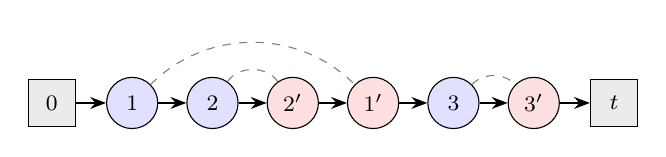
\begin{tikzpicture}[
  every node/.style={font=\footnotesize},
  pnode/.style={circle,draw,fill=blue!12,minimum size=6.5mm,inner sep=0pt},
  dnode/.style={circle,draw,fill=red!12,minimum size=6.5mm,inner sep=0pt},
  dep/.style={rectangle,draw,fill=black!8,minimum size=6mm,inner sep=2pt},
  arc/.style={-{Stealth[length=2mm]},thick}
]
\def\dx{1.02}
\node[dep] (s) at (0,0) {0};
\node[pnode] (p1) at (1*\dx,0) {1};
\node[pnode] (p2) at (2*\dx,0) {2};
\node[dnode] (d2) at (3*\dx,0) {$2'$};
\node[dnode] (d1) at (4*\dx,0) {$1'$};
\node[pnode] (p3) at (5*\dx,0) {3};
\node[dnode] (d3) at (6*\dx,0) {$3'$};
\node[dep] (t) at (7*\dx,0) {$t$};

\foreach \a/\b in {s/p1,p1/p2,p2/d2,d2/d1,d1/p3,p3/d3,d3/t}
  \draw[arc] (\a) -- (\b);

% precedence/LIFO arcs (pairing) drawn as arcs above
\draw[dashed,gray] (p1) to[bend left=45] (d1);
\draw[dashed,gray] (p2) to[bend left=55] (d2);
\draw[dashed,gray] (p3) to[bend left=45] (d3);
\end{tikzpicture}
\caption{Estructura de palíndromos anidados en una solución factible del TSPPDL con tres solicitudes. Los nodos azules son recogidas ($i$) y los rojos entregas ($i'$). Las solicitudes 1 y 2 forman un palíndromo anidado (P1, P2, D2, D1) y la solicitud 3 forma un palíndromo simple. Los arcos punteados emparejan cada recogida con su entrega; su no cruzamiento garantiza la factibilidad LIFO. Figura de elaboración propia.}
\label{fig:lifo}
\end{figure}

\subsection{Formulación de programación lineal entera}
Presentamos la formulación de tres índices reducida a las variables de arco, denotada TSPPDL3 en \cite{cordeau2010}, por ser compacta y la más efectiva reportada. A cada arco $(i,j)\in A$ se asocia una variable binaria $x_{ij}$ que toma valor $1$ si y solo si el nodo $j$ se visita inmediatamente después del nodo $i$. Se emplea la notación estándar $x(S)=\sum_{i,j\in S}x_{ij}$ para el número de arcos internos a un subconjunto $S$, y $x(\delta^{+}(i))$, $x(\delta^{-}(i))$ para los arcos que salen y entran de un nodo $i$, respectivamente. Además, $x(i,S)=\sum_{j\in S}x_{ij}$ y $x(S,i)=\sum_{j\in S}x_{ji}$.

La función objetivo minimiza el costo total de ruteo:
\begin{equation}
\min \sum_{i\in N}\sum_{j\in N} c_{ij}\,x_{ij}. \label{eq:obj}
\end{equation}

Las restricciones de grado aseguran que cada nodo de recogida y entrega se visite exactamente una vez:
\begin{align}
x(\delta^{+}(i)) &= 1 && \forall i\in P\cup D\cup\{0\}, \label{eq:out}\\
x(\delta^{-}(i)) &= 1 && \forall i\in P\cup D\cup\{2n+1\}. \label{eq:in}
\end{align}

Las restricciones de eliminación de subtoures garantizan la conectividad de la ruta:
\begin{equation}
x(S) \le |S|-1 \qquad \forall S\subseteq P\cup D,\ |S|\ge 2. \label{eq:subtour}
\end{equation}

Las restricciones de precedencia imponen que la recogida anteceda a su entrega. Sea $\mathcal{S}$ la colección de subconjuntos $S\subset N$ tales que $0\in S$, $2n+1\in S$ y existe un nodo $i$ con $i\notin S$ y $n+i\in S$:
\begin{equation}
x(S) \le |S|-2 \qquad \forall S\in \mathcal{S}. \label{eq:prec}
\end{equation}

Finalmente, la política LIFO se expresa únicamente en términos de las variables $x_{ij}$. Sea $\Gamma$ la colección de subconjuntos $S\subset P\cup D$ para los que existe al menos una solicitud $j$ tal que exactamente uno de los nodos $j$ o $n+j$ pertenece a $S$. Entonces:
\begin{equation}
x(i,S)+x(S)+x(S,n+i) \le |S| \quad \forall S\in\Gamma,\ i,n+i\notin S,\ i\in P. \label{eq:lifo}
\end{equation}
junto con la integralidad $x_{ij}\in\{0,1\}$ para todo $(i,j)\in A$.

La intuición de \eqref{eq:lifo} es la siguiente: si se intentara entrar a un subconjunto $S$ desde la recogida $i$ y salir hacia la entrega $n+i$, atravesando un conjunto de nodos que rompe la estructura de pila, se violaría la disciplina LIFO; la desigualdad prohíbe precisamente esa configuración \cite{cordeau2010}. El número de restricciones \eqref{eq:prec} y \eqref{eq:lifo} es exponencial, por lo que en la práctica se separan dinámicamente dentro de un esquema de ramificación y corte (\textit{branch-and-cut}).

\section{Complejidad y aplicaciones}\label{sec:comp}

\subsection{Origen histórico del problema}
El TSPPDL fue mencionado por primera vez por Ladany y Mehrez en 1984, quienes describieron un problema real de distribución en Israel en el que un vehículo con acceso trasero único debía servir un conjunto de clientes bajo la restricción de que la carga no podía reordenarse \cite{cordeau2010}. Sin embargo, estos autores no propusieron una formulación matemática formal ni un algoritmo de propósito general; su contribución fue de carácter descriptivo y su solución se basó en enumeración para instancias muy pequeñas (típicamente $n=5$). La estructura teórica del problema —incluyendo su relación con grafos planos y permutaciones de pila— fue analizada independientemente por Volchenkov en 1982 en el contexto de la gestión de memoria de pila en computadoras \cite{cordeau2010}. Las primeras heurísticas publicadas explícitamente para el TSPPDL aparecieron en la década de 1990 con los trabajos de Pacheco, y la primera formulación MILP rigurosa y el primer algoritmo exacto competitivo fueron propuestos por Carrabs, Cerulli y Cordeau en 2007 \cite{carrabs2007bb}, siendo superados posteriormente por el branch-and-cut de Cordeau et al.\ en 2010 \cite{cordeau2010}, que constituye hasta hoy la referencia exacta del estado del arte.

\subsection{Complejidad computacional}
El TSPPDL pertenece a la clase NP-hard. La demostración formal fue establecida por Cordeau et al.\ \cite{cordeau2010} mediante una reducción polinomial desde el \textit{Asymmetric Traveling Salesman Problem} (ATSP), que es NP-hard por reducción desde el problema de la ruta hamiltoniana. La reducción construye una instancia del TSPPDL a partir de cualquier instancia del ATSP de la siguiente forma: a cada cliente $i$ del ATSP se le asocian dos nodos, un nodo de recogida $i$ y un nodo de entrega $n+i$, y la matriz de costos se modifica de modo que el único camino de costo finito obliga al vehículo a visitar $i$ inmediatamente antes que $n+i$, colapsando efectivamente cada solicitud en un único cliente del ATSP original. Dado que cualquier solución óptima al ATSP puede construirse en tiempo polinomial a partir de una solución al TSPPDL y viceversa, la NP-hardness se hereda directamente.

Una consecuencia práctica de esta complejidad es el reducido tamaño de las instancias resolubles de forma exacta. El número de soluciones factibles crece de manera explosiva: Cordeau et al.\ \cite{cordeau2010} establecen una recursión cerrada que muestra que, aunque el LIFO reduce el espacio de búsqueda frente al TSPPD (por ejemplo, de $8{,}2\times10^{10}$ a $57{,}6$ millones de soluciones para $n=8$), el crecimiento sigue siendo superexponencial. Los mejores algoritmos exactos resuelven a optimalidad instancias de hasta $25$ solicitudes ($52$ nodos), mientras que casi todas las instancias de hasta $17$ solicitudes se resuelven en menos de un minuto \cite{cordeau2010}. Para tamaños mayores, propios de la operación real, se vuelven indispensables los enfoques heurísticos y metaheurísticos \cite{li2011,cheang2012}.

\subsection{Aplicaciones reales}
El TSPPDL y sus variantes modelan diversas operaciones industriales y logísticas:

\begin{enumerate}
\item \textbf{Logística urbana y mensajería}: el transporte puerta a puerta de paquetes con vehículos de carga trasera, donde el reordenamiento de la carga es costoso o inviable, se ajusta naturalmente a la disciplina LIFO \cite{cordeau2010,andriansyah2018}.
\item \textbf{Manufactura y vehículos guiados automáticamente (AGV)}: Levitin y Abezgaouz \cite{levitin2003} estudian el ruteo de AGV de carga múltiple que distribuyen materias primas y semielaborados entre estaciones de trabajo. Como el AGV emplea una pila sin acceso aleatorio, las operaciones de carga y descarga deben respetar el orden LIFO.
\item \textbf{Transporte de ítems voluminosos, frágiles o peligrosos}: evitar la reorganización de la carga es prioritario cuando los objetos son grandes, pesados o requieren manipulación cuidadosa; aquí el costo de reordenar domina sobre la distancia adicional inducida por la restricción \cite{li2011,ruan2021}.
\end{enumerate}

Variantes posteriores extienden el problema a múltiples vehículos y restricciones de distancia \cite{cheang2012,gao2011}, ventanas de tiempo \cite{liu2019}, número limitado de vehículos \cite{andriansyah2018} y escenarios dinámicos \cite{du2023}, ampliando el rango de aplicaciones cubiertas.

\section{Estado del arte de los métodos de resolución}\label{sec:sota}
Esta sección sintetiza el panorama de enfoques de resolución para el TSPPDL, organizado en métodos exactos, heurísticos, metaheurísticos y de aprendizaje. Al final se sitúa a LKH-3 dentro de este panorama.

\subsection{Métodos exactos}
El TSPPDL fue mencionado por primera vez por Ladany y Mehrez en 1984, quienes describieron un problema real de distribución en Israel sin proponer una formulación matemática \cite{cordeau2010}. Los primeros algoritmos exactos fueron métodos de ramificación y acotamiento (\textit{branch-and-bound}) basados en relajaciones del TSP. Carrabs, Cerulli y Cordeau \cite{carrabs2007bb} propusieron un algoritmo aditivo de ramificación y acotamiento que emplea cotas inferiores basadas en relajaciones del problema de asignación y del problema de la $r$-arborescencia de expansión mínima, junto con filtros que eliminan arcos inviables en cada nodo del árbol de enumeración; este método resuelve la mayoría de las instancias con $15$ solicitudes y algunas con hasta $21$.

El estado del arte exacto lo establece el algoritmo de ramificación y corte de Cordeau et al.\ \cite{cordeau2010}, que constituye la referencia obligada del problema. Los autores proponen tres formulaciones de programación lineal entera y varias familias de desigualdades válidas —entre ellas las novedosas \textit{hamburger inequalities}, específicas de la estructura LIFO— que se separan dinámicamente. La formulación TSPPDL3 con separación de cortes resuelve a optimalidad $37$ de $45$ instancias en menos de una hora de CPU, supera al \textit{branch-and-bound} previo y resuelve la instancia más grande conocida de $25$ solicitudes. Cabe notar que estos métodos exactos descansan sobre una representación basada en listas de vértices, cuya verificación de factibilidad es costosa.

\subsection{Heurísticos constructivos y de búsqueda local}
Dado el límite práctico de los métodos exactos, la literatura ha desarrollado heurísticas para instancias grandes. Trabajos tempranos de Pacheco y de Cassani propusieron heurísticas voraces e intercambios de tipo Or-opt para el TSPPDL no capacitado, reportando resultados sobre instancias de hasta $120$ clientes \cite{cordeau2010}. Estos enfoques se basan en operadores de intercambio que reorganizan localmente la secuencia de visitas preservando la factibilidad LIFO.

Un avance conceptual significativo fue la introducción de la representación en árbol de las soluciones factibles. Tu et al.\ \cite{tu2010} y, en su versión extendida, Li et al.\ \cite{li2011} demostraron que las soluciones factibles del TSPPDL pueden representarse mediante árboles, lo que simplifica notablemente la verificación de factibilidad respecto de las listas de vértices. Sobre esta estructura definieron operadores de búsqueda que respetan automáticamente las restricciones de precedencia y LIFO.

\subsection{Metaheurísticas}
Las metaheurísticas constituyen el enfoque dominante para instancias de tamaño realista. Carrabs et al.\ desarrollaron nuevos operadores de intercambio y una búsqueda de vecindario variable (VNS) que reportó resultados sobre instancias de hasta $375$ solicitudes \cite{cordeau2010,li2011}. Posteriormente, la VNS basada en la representación en árbol de Li et al.\ \cite{li2011} superó a estos métodos tanto en calidad de solución como en tiempo de cómputo, reproduciendo los operadores clásicos sobre la nueva estructura e incorporando operadores adicionales.

Las extensiones del problema motivaron nuevas metaheurísticas. Cheang et al.\ \cite{cheang2012} y Gao et al.\ \cite{gao2011} abordaron la variante con múltiples vehículos y restricciones de distancia (MTSPPD-LD), proponiendo operadores de vecindario, recocido simulado, búsqueda tabú probabilística y VNS, junto con un componente de programación dinámica para resolver óptimamente subproblemas TSPPDL. Para la variante con ventanas de tiempo, Liu et al.\ \cite{liu2019} propusieron un marco de descomposición y reconstrucción que paraleliza búsquedas tabú sobre subsoluciones, mejorando más del $85\%$ de las mejores soluciones conocidas en instancias de hasta $300$ solicitudes. En el escenario dinámico, Du et al.\ \cite{du2023} introdujeron un enfoque de optimización jerárquica con operadores basados en bloques que respetan la restricción LIFO, validado sobre instancias reales.

Es ilustrativo contrastar la disciplina LIFO con la política opuesta First-In-First-Out (FIFO): Erdo\u{g}an et al.\ \cite{erdogan2009} formularon y resolvieron el TSPPDF, mostrando que ambas variantes comparten estructura de familia pero difieren en los operadores de factibilidad requeridos. Asimismo, restricciones de carga más ricas —como el apilamiento tridimensional— han sido tratadas mediante algoritmos genéticos que incorporan mejoras de tipo Lin--Kernighan en la ruta de entrega \cite{ruan2021}.

\subsection{Enfoques de aprendizaje}
En los últimos años, el aprendizaje por refuerzo profundo (DRL) ha emergido como una vía prometedora para problemas de ruteo. Zong et al.\ \cite{zong2025} presentan un panorama exhaustivo de DRL aplicado a servicios logísticos impulsados por la demanda, destacando que estos métodos aprenden modelos paramétricos sin depender de supuestos específicos del problema y optimizan efectos de largo plazo mediante decisiones secuenciales. Aplicaciones recientes de DRL al ruteo de última milla, integrando transporte público y condiciones de tráfico, ilustran la capacidad de estos enfoques para operar en entornos urbanos complejos \cite{elamrani2025}. No obstante, la incorporación explícita de restricciones de carga LIFO dentro de arquitecturas de aprendizaje permanece poco explorada, lo que constituye una brecha relevante.

\section{El solver LKH-3 aplicado al TSPPDL}\label{sec:lkh}
El solver Lin--Kernighan--Helsgaun (LKH) es uno de los resolvedores heurísticos más efectivos para el TSP, basado en la búsqueda local de profundidad variable de Lin y Kernighan \cite{helsgaun2017}. Su versión LKH-3 extiende el algoritmo para tratar una amplia familia de problemas con restricciones, incluyendo variantes con precedencia, capacidad, ventanas de tiempo y recogida-entrega \cite{helsgaun2017}.

La idea central de LKH-3 es transformar el problema restringido en una instancia de TSP simétrico estándar, sobre la cual opera el motor de búsqueda local original. Las restricciones que no pueden codificarse directamente en la estructura del TSP se manejan mediante \textit{penalizaciones}: a cada solución candidata se le asocia, además del costo de la ruta, una penalización proporcional al grado de violación de las restricciones. El algoritmo minimiza primero la penalización y, entre soluciones de igual penalización, minimiza la distancia. De este modo, las restricciones de precedencia y de carga propias del TSPPDL se incorporan como términos penalizadores que guían la búsqueda hacia soluciones factibles \cite{helsgaun2017}.

Para los problemas de recogida y entrega, LKH-3 representa cada par mediante nodos asociados y emplea mecanismos que preservan la relación de precedencia durante los movimientos de la búsqueda de profundidad variable. Helsgaun reporta que LKH-3 obtiene soluciones de calidad equivalente a las mejores conocidas en numerosos conjuntos de instancias de referencia, y en algunos casos encuentra nuevas mejores soluciones \cite{helsgaun2017}. Su posición en el panorama es, por tanto, la de un resolvedor heurístico de propósito general y alto rendimiento: a diferencia de las metaheurísticas especializadas en el TSPPDL —que explotan estructuras como la representación en árbol \cite{li2011}— LKH-3 ofrece un marco unificado capaz de abordar múltiples variantes con una sola implementación, a cambio de no incorporar el conocimiento estructural específico del problema.

\section{Discusión y trabajo futuro}\label{sec:disc}
La revisión realizada permite identificar varias brechas abiertas y tendencias recientes en el estudio del TSPPDL.

En primer lugar, persiste una brecha pronunciada entre el tamaño de las instancias resolubles de forma exacta —del orden de $25$ solicitudes \cite{cordeau2010}— y las dimensiones requeridas en la operación real, que las metaheurísticas abordan sin garantías de optimalidad \cite{li2011,cheang2012}. Cerrar esta brecha, ya sea mediante formulaciones más fuertes, nuevas familias de desigualdades válidas o esquemas de descomposición, sigue siendo un desafío vigente.

En segundo lugar, las variantes más cercanas a la práctica —múltiples vehículos, ventanas de tiempo, restricciones de distancia y escenarios dinámicos \cite{cheang2012,liu2019,du2023}— han recibido atención creciente en los últimos cinco años, lo que sugiere un desplazamiento del interés desde el caso canónico de un único vehículo hacia formulaciones más realistas y de mayor complejidad combinatoria.

En tercer lugar, la integración de restricciones de carga LIFO dentro de enfoques de aprendizaje por refuerzo profundo permanece escasamente explorada \cite{zong2025,elamrani2025}. Mientras que el DRL ha mostrado resultados notables en problemas de ruteo sin restricciones de apilamiento, la codificación de la disciplina de pila en el espacio de estados y acciones, así como el diseño de funciones de recompensa que penalicen las violaciones LIFO, constituyen direcciones de investigación prometedoras.

Finalmente, respecto del rol de LKH-3, su carácter de resolvedor unificado lo convierte en una línea base valiosa para comparar nuevos métodos sobre múltiples variantes, aunque su rendimiento relativo frente a heurísticas que explotan la estructura específica del TSPPDL —como la representación en árbol \cite{li2011}— en instancias de gran tamaño merece un estudio empírico sistemático.

\section*{Declaración de uso de IA}
En la elaboración de este trabajo se utilizó la herramienta de IA generativa Claude (Anthropic) como apoyo en las siguientes tareas: organización de la estructura del documento conforme a la plantilla IEEE, asistencia en la redacción y edición del estilo, y síntesis comparativa de la literatura previamente seleccionada y leída por el grupo. Todas las referencias citadas fueron verificadas y leídas por al menos un integrante del grupo. La estructura analítica, el posicionamiento crítico de LKH-3 y la discusión son obra del grupo. La IA no se empleó para generar referencias ni para sustituir el análisis propio.

\begin{thebibliography}{00}
\bibitem{cordeau2010} J.-F. Cordeau, M. Iori, G. Laporte, and J. J. Salazar González, ``A branch-and-cut algorithm for the pickup and delivery traveling salesman problem with LIFO loading,'' Networks, vol. 55, no. 1, pp. 46--59, 2010.
\bibitem{carrabs2007bb} F. Carrabs, R. Cerulli, and J.-F. Cordeau, ``An additive branch-and-bound algorithm for the pickup and delivery traveling salesman problem with LIFO loading,'' INFOR: Inf. Syst. Oper. Res., vol. 45, no. 4, pp. 223--238, 2007.
\bibitem{li2011} Y. Li, A. Lim, W.-C. Oon, H. Qin, and D. Tu, ``The tree representation for the pickup and delivery traveling salesman problem with LIFO loading,'' Eur. J. Oper. Res., vol. 212, no. 3, pp. 482--496, 2011.
\bibitem{tu2010} D. Tu, S. Guo, H. Qin, W.-C. Oon, and A. Lim, ``The tree representation of feasible solutions for the TSP with pickup and delivery and LIFO loading,'' in Proc. 24th AAAI Conf. Artif. Intell. (AAAI-10), 2010, pp. 191--196.
\bibitem{cheang2012} B. Cheang, X. Gao, A. Lim, H. Qin, and W. Zhu, ``Multiple pickup and delivery traveling salesman problem with last-in-first-out loading and distance constraints,'' Eur. J. Oper. Res., vol. 223, no. 1, pp. 60--75, 2012.
\bibitem{gao2011} X. Gao, A. Lim, H. Qin, and W. Zhu, ``Multiple pickup and delivery TSP with LIFO and distance constraints: a VNS approach,'' in Proc. 24th Int. Conf. Ind. Eng. Other Appl. Appl. Intell. Syst. (IEA/AIE), LNAI 6704, 2011, pp. 193--202.
\bibitem{levitin2003} G. Levitin and R. Abezgaouz, ``Optimal routing of multiple-load AGV subject to LIFO loading constraints,'' Comput. Oper. Res., vol. 30, no. 3, pp. 397--410, 2003.
\bibitem{liu2019} F. Liu, M. Gui, C. Yi, and Y. Lan, ``A fast decomposition and reconstruction framework for the pickup and delivery problem with time windows and LIFO loading,'' IEEE Access, vol. 7, pp. 71813--71826, 2019.
\bibitem{du2023} J. Du, Z. Zhang, X. Wang, and H. C. Lau, ``A hierarchical optimization approach for dynamic pickup and delivery problem with LIFO constraints,'' Transp. Res. Part E: Logist. Transp. Rev., vol. 175, art. 103131, 2023.
\bibitem{andriansyah2018} Andriansyah, N. Prasanti, and P. D. Sentia, ``Pickup and delivery problem with LIFO, time duration, and limited vehicle number,'' MATEC Web Conf., vol. 204, art. 07003, 2018.
\bibitem{erdogan2009} G. Erdo\u{g}an, J.-F. Cordeau, and G. Laporte, ``The pickup and delivery traveling salesman problem with first-in-first-out loading,'' Comput. Oper. Res., vol. 36, no. 6, pp. 1800--1808, 2009.
\bibitem{ruan2021} M. Ruan, C. Shen, J. Tang, C. Qi, and S. Qiu, ``A double traveling salesman problem with three-dimensional loading constraints for bulky item delivery,'' IEEE Access, vol. 9, pp. 13052--13063, 2021.
\bibitem{zong2025} Z. Zong, T. Feng, J. Wang, T. Xia, and Y. Li, ``Deep reinforcement learning for demand-driven services in logistics and transportation systems: a survey,'' ACM Trans. Knowl. Discov. Data, vol. 19, no. 4, art. 89, 2025.
\bibitem{elamrani2025} A. M. El Amrani, M. Fri, O. Benmoussa, and N. Rouky, ``A deep reinforcement learning framework for last-mile delivery with public transport and traffic-aware integration: a case study in Casablanca,'' Infrastructures, vol. 10, no. 5, art. 112, 2025.
\bibitem{helsgaun2017} K. Helsgaun, ``An extension of the Lin-Kernighan-Helsgaun TSP solver for constrained traveling salesman and vehicle routing problems,'' Roskilde Univ., Roskilde, Denmark, Tech. Rep., Dec. 2017.
\bibitem{savelsbergh1995} M. W. P. Savelsbergh and M. Sol, ``The general pickup and delivery problem,'' Transp. Sci., vol. 29, no. 1, pp. 17--29, 1995.
\bibitem{ruland1997} K. S. Ruland and E. Y. Rodin, ``The pickup and delivery problem: faces and branch-and-cut algorithm,'' Comput. Math. Appl., vol. 33, no. 12, pp. 1--13, 1997.
\end{thebibliography}

\end{document}
